\documentclass{article}
\usepackage[headheight=40pt, textheight=560pt]{geometry}
\usepackage{paralist}
\usepackage{scalerel,amssymb}
\usepackage{amsmath}
\usepackage{colortbl}
\usepackage{array}
\usepackage{multirow}
\usepackage{blindtext}
\usepackage{reledmac}
\usepackage{changepage}

\usepackage{pgfplots}
\usepackage{tikz}
\usetikzlibrary{positioning}
\usetikzlibrary{shapes.geometric, arrows}
\tikzstyle{arrow} = [thick,->,>=stealth]

\usepackage{graphicx}
\usepackage{stix}

\newcommand{\tableflip}{$($\rotatebox{45}{$\smile$}$^{\circ}\smwhtsquare^{\circ})\rotatebox{45}{$\smile$}\mkern-6mu\frown$\raisebox{0.5ex}{$\bot$}$\mkern-3.5mu-\mkern-3.5mu$\raisebox{0.5ex}{$\bot$}}

\usepackage{fancyhdr}
\fancyhead[L]{
	\begin{tabular}{lll}
		\begin{tabular}{l}
			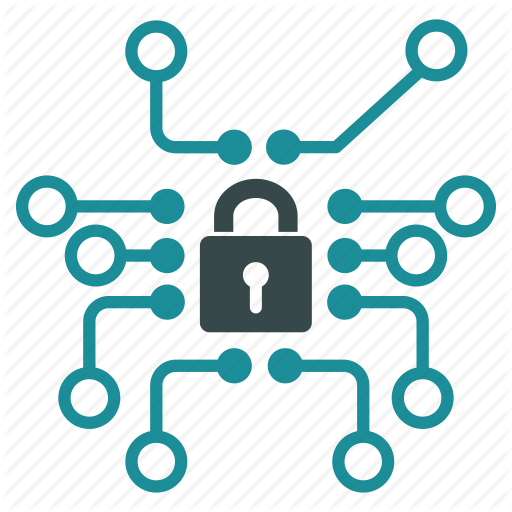
\includegraphics[scale=0.1]{security_lock}
		\end{tabular}	
		&
		\begin{tabular}{l}
			\LARGE \textbf{Cryptography} \\
			\Large \textsc{Zusammenfassung}
		\end{tabular}
		&
		\begin{tabular}{l}
			\tableflip
		\end{tabular}
	\end{tabular}
}
\fancyhead[R]{16-124-836 \\
Marcel \textsc{Zauder}}
\renewcommand{\headrulewidth}{0.4pt}
\fancyfoot[C]{\thepage}
\renewcommand{\footrulewidth}{0.4pt}

\usepackage{hyperref}

\begin{document}
	\pagestyle{fancy}
	\section{One Time Pad}
		\begin{adjustwidth*}{2em}{}
			\subsection{What is [\textsc{not}] \textsc{Cryptography}}
			\begin{adjustwidth*}{2em}{}
				\subsubsection{Introduction}
					\begin{adjustwidth*}{2em}{4em}
						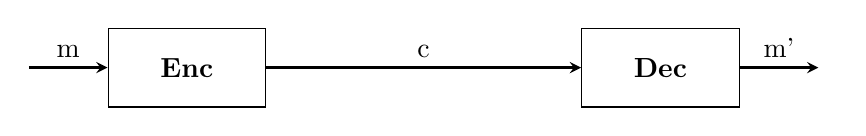
\begin{tikzpicture}
							\coordinate (start);
							
							%Nodes
							\node (rect) [draw,thin,minimum width=2cm,minimum height=1cm, right=of start] (Enc) {\textsc{\textbf{Enc}}};
							\node (rect) [draw,thin,minimum width=2cm,minimum height=1cm, right=4cm of Enc] (Dec) {\textsc{\textbf{Dec}}};
							\node [right=of Dec] (stop) {};
							
							%Lines
							\draw[arrow] (start) -- node[ anchor=south ]{m} (Enc.west);
							\draw[arrow] (Enc.east) -- node[ anchor=south ]{c} (Dec.west);
							\draw[arrow] (Dec.east) -- node[ anchor=south ]{m'} (stop.west);
							
						\end{tikzpicture}
					\end{adjustwidth*}
				\subsubsection{Kerckhoff's principle}
				\begin{adjustwidth*}{2em}{4em}
					\textit{The method must not be required to be secret, and it must be able to fall into the enemy's hands without causing any inconvenience.} \\ \\
					So if the algorithm do not need to be secret, there must be additional information in the system, which is kept secret from any \textsc{Eavesdropper}. This information is called a \textbf{(secret) key}. \\ \\
					\begin{tikzpicture}							
							%Nodes
							\node (rect) [draw,thin,minimum width=2cm,minimum height=1cm, right=of start] (KeyGen) {\textsc{\textbf{KeyGen()}}};
							\node [below=of KeyGen] (start) {};
							\node (rect) [draw,thin,minimum width=2cm,minimum height=1cm, right=of start] (Enc) {\textsc{\textbf{Enc}}};
							\node (rect) [draw,thin,minimum width=2cm,minimum height=1cm, right=4cm of Enc] (Dec) {\textsc{\textbf{Dec}}};
							\node [right=of Dec] (stop) {};
							
							%Lines
							\draw[arrow] (KeyGen.east) -| node[ anchor=south ]{k} (Enc.north);
							\draw[arrow] (KeyGen.east) -| node[ anchor=south ]{k} (Dec.north);
							\draw[arrow] (start) -- node[ anchor=south ]{m} (Enc.west);
							\draw[arrow] (Enc.east) -- node[ anchor=south ]{c} (Dec.west);
							\draw[arrow] (Dec.east) -- node[ anchor=south ]{m'} (stop.west);
							
						\end{tikzpicture}
				\end{adjustwidth*}
			\end{adjustwidth*}
		\end{adjustwidth*}
		\begin{adjustwidth*}{2em}{}
			\subsection{Specifics of One Time Pad}
		\end{adjustwidth*}
	
\end{document}